
\section{Choosing features for Neural Network model}
A major part of this project was dedicated to finding the correct way to represent the collected user data in the form of a graph. The most interesting of these representations are discussed in this section.


\subsection{Graph creation and feature encoding}
The input for graph creation consists of two main parts, the duration of time between individual key presses, and the character of the key that was pressed.
A natural way to represent such input was to map each unique character in the input sequence to a node in the graph. 
Directed edges were added between nodes that represent characters appearing after each other in the input sequence. Each time the same pair of characters appears in the input text, it maps to the same edge. For each such pair, the duration is added to a list of attributes associated with that edge, which will be aggregated in later stages into a form suitable for the GCN model. It is also possible to model such pairs using a multiedge graph, as such models have been shown to perform well in other domains. However, this approach was not considered in this study. 

A simple visualization of such graph, created from the input text: "Cat and dog and .", with arbitrary keystroke durations, is shown in figure \ref{fig:example_graph}.

\begin{figure}[H]
	\centering
	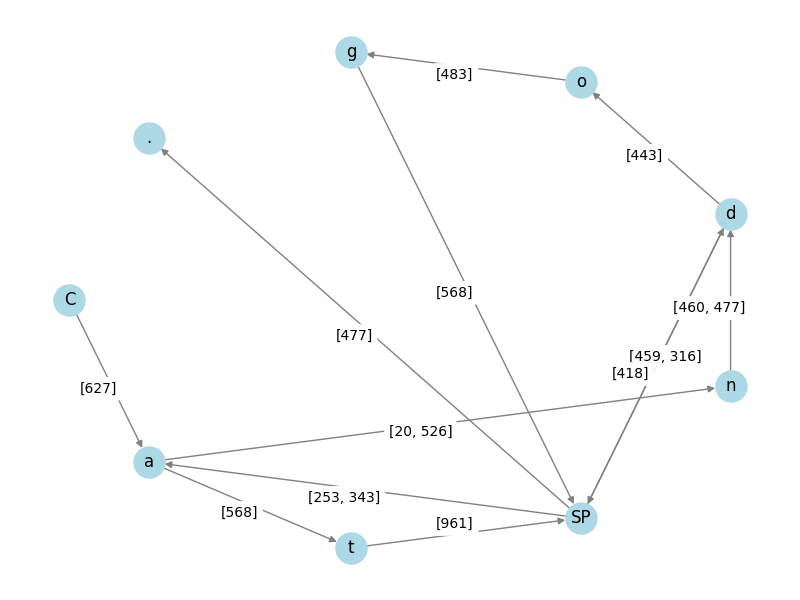
\includegraphics[width=.65\textwidth]{images/graph_with_edge.png} 	
	\caption{Graph for the sequence "Cat and dog and ."}
	\label{fig:example_graph}
\end{figure}


The structure of the resulting graph highly depends on the length of the input sequence. A shorter sequences produce smaller and sparser graphs, while a longer input sequences result in graphs with more nodes and edges. An example taken from the training dataset is shown below: one graph with 40 characters and another with 70. Edge weights have been omitted for clarity.

\begin{figure}[H]
	\centering
	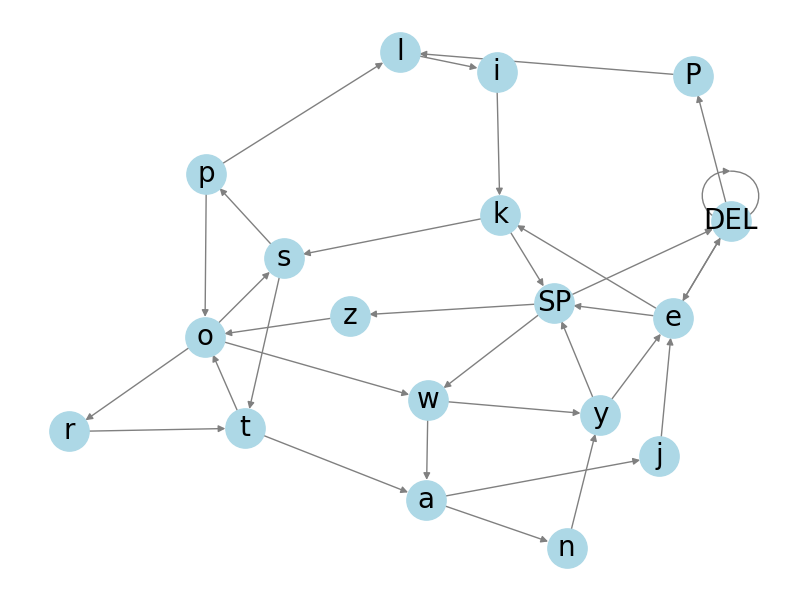
\includegraphics[width=0.49\textwidth]{images/len40_graph_other_layout.png}
	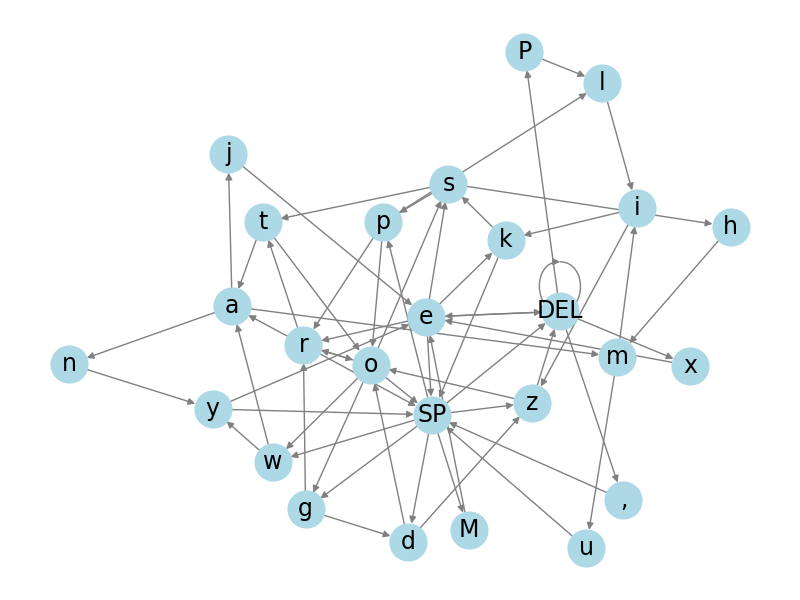
\includegraphics[width=0.49\textwidth]{images/better_70_char_graph.png}
	\caption{Comparison of graphs constructed with different input sequence lengths of 40 and 70.}%
	\label{fig:multiple graphs}%
\end{figure}


\subsection{Edge attributes encoding}
In order for the graph to be a valid input for a GCN network, edge attributes need to be converted into node features. Two methods were identified to encode this information into node features. For each node $i$:
\begin{enumerate}
	\item Two values representing the average duration before and after the key represented by $i$ was pressed.
	\item A two-dimensional vector of values with a size of [number of allowed characters, 2]. Each key that appears in the input is assigned a number. The $n$-th row in the vector corresponds to a node, with a key assigned the number $n$, now called node $j$. The $n$-th row contains two values: the average duration on the edge from $i$ to $j$ and the average duration on the edge from $j$ to $i$. The values for which edges do not exist were assigned 0.
\end{enumerate}
The key difference between these two approaches is the level of aggregation. Method $1$ aggregates all the edge information into two values, while method $2$ aggregates it into a vector of values, although it imposes some limitations, such as assigning each key a unique index into this input vector. Furthermore, method $2$ increases the overall size of the input data and the complexity of the model.


\subsection{Character attributes encoding}
\label{Base_letter_representation}
As this project focuses on recognizing users of the Polish language, the character encodings were designed to make use of this fact. For encoding purposes, characters were divided into several groups:
\begin{itemize}
	\item Letters -- characters \textit{a-z}, including diacritics.
	\item Numbers -- characters \textit{0-9}.
	\item Special characters -- \textit{space}, \textit{tab}, \textit{newline}, \textit{backspace}, \textit{dot}, \textit{comma}, \textit{exclamation mark}, \textit{question mark}.
	\item Symbols -- \textit{*}, \textit{\#}, \textit{@}, \textit{:}, \textit{;},   \textit{'}, \textit{"}, \textit{(}, \textit{)}, \textit{[}, \textit{]}, \textit{\{}, \textit{\}}, \textless, \textgreater, \textit{/}, \textit{$\backslash$}, \textit{|}, \&, \%, \textit{\$}, \textit{\^}, \~, \textit{\_}, \textit{+}, \textit{-}, \textit{=}. 
	\item Others -- all other symbols.
\end{itemize}
Similarly, there is more than one way to encode key information into node features.
Three methods were considered, all of which are variations of one-hot encoding of keys:
\begin{enumerate}
	\item Full One-Hot Encoding. Each unique cased character is mapped to a different column in the vector, except for characters in the \textit{Others} group, which are mapped to an additional column.
	\item Compact Alphabet Encoding. A more compact version of the \textit{Full One-Hot Encoding}. One-hot encoding is used for cased \textit{Letters} and \textit{Special characters}. \textit{Numbers} are grouped and mapped to a single column in the vector.
	\textit{Symbols} and \textit{Others} are grouped together and mapped to another column in the vector.
	\item Normalized Base Letter Encoding. \textit{Letters} are simplified by converting them to lowercase and removing diacritical marks. These transformed letters are encoded in a one-hot vector. \textit{Numbers} are mapped to a single column in the vector, \textit{Symbols} and \textit{Others} are mapped in the same way as in the \textit{Compact Alphabet Encoding}. Two additional columns are added to indicate whether the original character was capitalized and if it had a diacritical mark.
\end{enumerate}


These methods differ by their degree of aggregation. Methods $2$ and $3$ group certain letters together, mapping multiple characters to the same values, while method $1$ provides a unique, one-hot encoded identifier for each node. Node identifiers have been found to help the model learn certain structures in the data \cite{you2021identityawaregraphneuralnetworks}. 

However, providing node identifiers as input features is effective only for a small and defined set of possible input nodes \cite{Lesk2024}. While this requirement appears to hold true for this specific task, it was found not to be the case.
Many letters that appear to be common are, in fact, infrequent in the dataset. This is especially true for capitalised letters. For example the letter \textit{'f'} appears 134 times, whereas \textit{'F'} appears only 6 times. This is even more true for symbols, many of which appear only once in the entire dataset, these being: \textit{'\{'}, \textit{'\%'}, \textit{'*'}, \textit{':'} and \textit{'\#'}.
This means that the behavior of the models would be unpredictable for nodes with such identifiers.
Method $2$ addresses the problem in the case of symbols and numbers. It does not, however help with processing infrequent capitalized diacritical letters. For example, \textit{'l'} appears 875 times, \textit{"ł"} 138 times, \textit{"L"} 10 times and \textit{"Ł"} only twice. With such a low number of occurances it is unlikely that the models could learn the relationship between these letters.
Method $3$ was specifically designed to deal with this problem, which is achieved by grouping them together. The extra columns still allow for distinguishing between varaints of the same letter, which is important because the time to input these symbol differs greatly, especially in the case of diacriticals, which take on average of 898 miliseconds to enter, compared to 346 for letters without diacritical marks.
Moreover, method $3$ directly exposes the use of diacritical marks and uppercase letters as features, which, in theory, could allow the model to learn the impact of these features independently of the base letters. 

\subsection{Feature selection: accelerometer data} \label{accel_subsection}
To improve the potential performance of the model, and to make further use of the capabilities of the mobile platform, accelerometer data was considered as an input feature for the model.
This portion of the input data consisted of three values, a measurement of the acceleration in the x, y and z axes at the moment a keystroke was registered. 
These values were aggregated as an average for each node. Although these models performed well during training, quickly achieving low loss values, they failed to generalize, performing worse on validation and test datasets. For this reason, accelerometer data was not used for training and evaluating models discussed later. Problems with accelerometer data have been mentioned in other studies \cite{maiorana2021}.

